\graphicspath{{introduction/fig/}}

\chapter{Introduction}
\label{chap:introduction}

\begin{quote}
    "We don't tell [computers] what to do, we give them examples... The problem is, sometimes we don't understand how it figured it out."\\ % <--- FORCED NEW LINE HERE
    \vspace{0.5em} % Adds a slightly larger vertical space after the quote text
    \hfill -- Jeff Dean, Head of Google AI \cite{Dean2017BlackBox}
\end{quote}


The prevalence of neural networks (NNs) has positioned them as a foundational technology in modern artificial intelligence. However, as their use has grown, so too has the focus on their inherent mechanistic limitations. Two of the most significant drawbacks of NNs are their lack of explainability---the "black-box" effect---and the immense computational cost required for training. With platforms like Hugging Face and GitHub providing access to over one million pre-trained models \cite{huggingface2024review} interest in these limitations has grown. Fueled by this enormous availability of models, a novel field, weight space learning, emerges as a promising area to further our understanding of these mechanistic limitations.



Weight space learning primarily focuses on developing methods to represent the high-dimensional weights of NN models in a lower-dimensional latent space, in order to facilitate further exploration of the weight space. The field generally considers two types of tasks: discriminative and generative.

In the discriminative application, models use the weights of already-trained models, with a specific collection of models referred to as a model zoo \cite{schurholt2022modelzoosdatasetdiverse}, as input to accurately predict meta-information about the original model \cite{unterthiner2021predictingneuralnetworkaccuracy}. The quality of weight space representation is often quantitatively measured by a simple Multi-layer perceptron (MLP)'s ability to predict this meta-information, conditioned only on the model's weight space representation. 

Common meta-information metrics investigated include predicting the model's final performance and the generalization gap (the difference between training and validation loss).\cite{salama2024datasetsizerecoverylora} has shown that weight embeddings can encode fundamental training characteristics, such as accurately recovering the size of the dataset on which the model was originally trained . These discriminative tasks serve the dual purpose of both validating the quality of the derived weight representations and possessing significant practical value.

In the generative application, researchers make use of varous methods to model the underlying distribution of NN weights $W$ conditioned on additional information or reference models $P(W\mid \dots)$. The process of sampling from this distruibution is what enables eintrely new weight generation

\cite{schurholt2022hyperrepresentationsgenerativemodelssampling} made use of an autoencoder with a bottleneck layer to generate a hyper-representations of various model zoo's. Expanding on this concept \cite{pmlr-v235-schurholt24a} makes use of a Sequential Autoencoder for Neural Embeddings (SANE) to improve the scaliablity of the method, allowing work on much larger models.

In order to model the distribution $P(W\mid \mathcal{D})$, \cite{bedionita2025instructionguidedautoregressiveneuralnetwork} use a Vector Quantized Variational Autoencoder (VQ-VAE), which takes in information about the dataset as part of the process of find latent weight representations.\cite{meynent2025structureenoughleveragingbehavior} models $P(W\mid R)$ through including the difference in behaviour between the reconstructed and original models in the process of learning model embeddings. 

While existing weight space learning methods have made significant progress, they typically focus on isolated aspects of the model learning process. Current approaches model either $P(W\mid \mathcal{D})$ or $P(W\mid R)$, but not both simultaneously. This represents a significant limitation: in practice, a model's weights are shaped by both the data it was trained and the results it achieved when training on a certain objective. Understanding the more complex joint relationship ---$P(W \mid D,R)$ --- is essential for both explaining model behavior and for generating new models with desired characteristics.

Contrastive learning has emerged as a powerful paradigm for learning unified representations across different modalities, as demonstrated by the success of models like CLIP \cite{radford2021learningtransferablevisualmodels} in bridging vision and language. A learned embedding space is learned through the use of a loss objective function which pulls related samples together in representation space, and pushes unrelated samples away from each other. This allows for the formation of a meaningful represnetation space, of heretogenous data types. It is this feaute of contrasitve learning which makes it particularly usefull to model the complex distribution $P(W \mid D,R)$ --- visual datasets, high-dimensional weight tensors, and performance metrics --- without requiring them to share the same native representation.

\begin{figure}[!t]
    \centering
    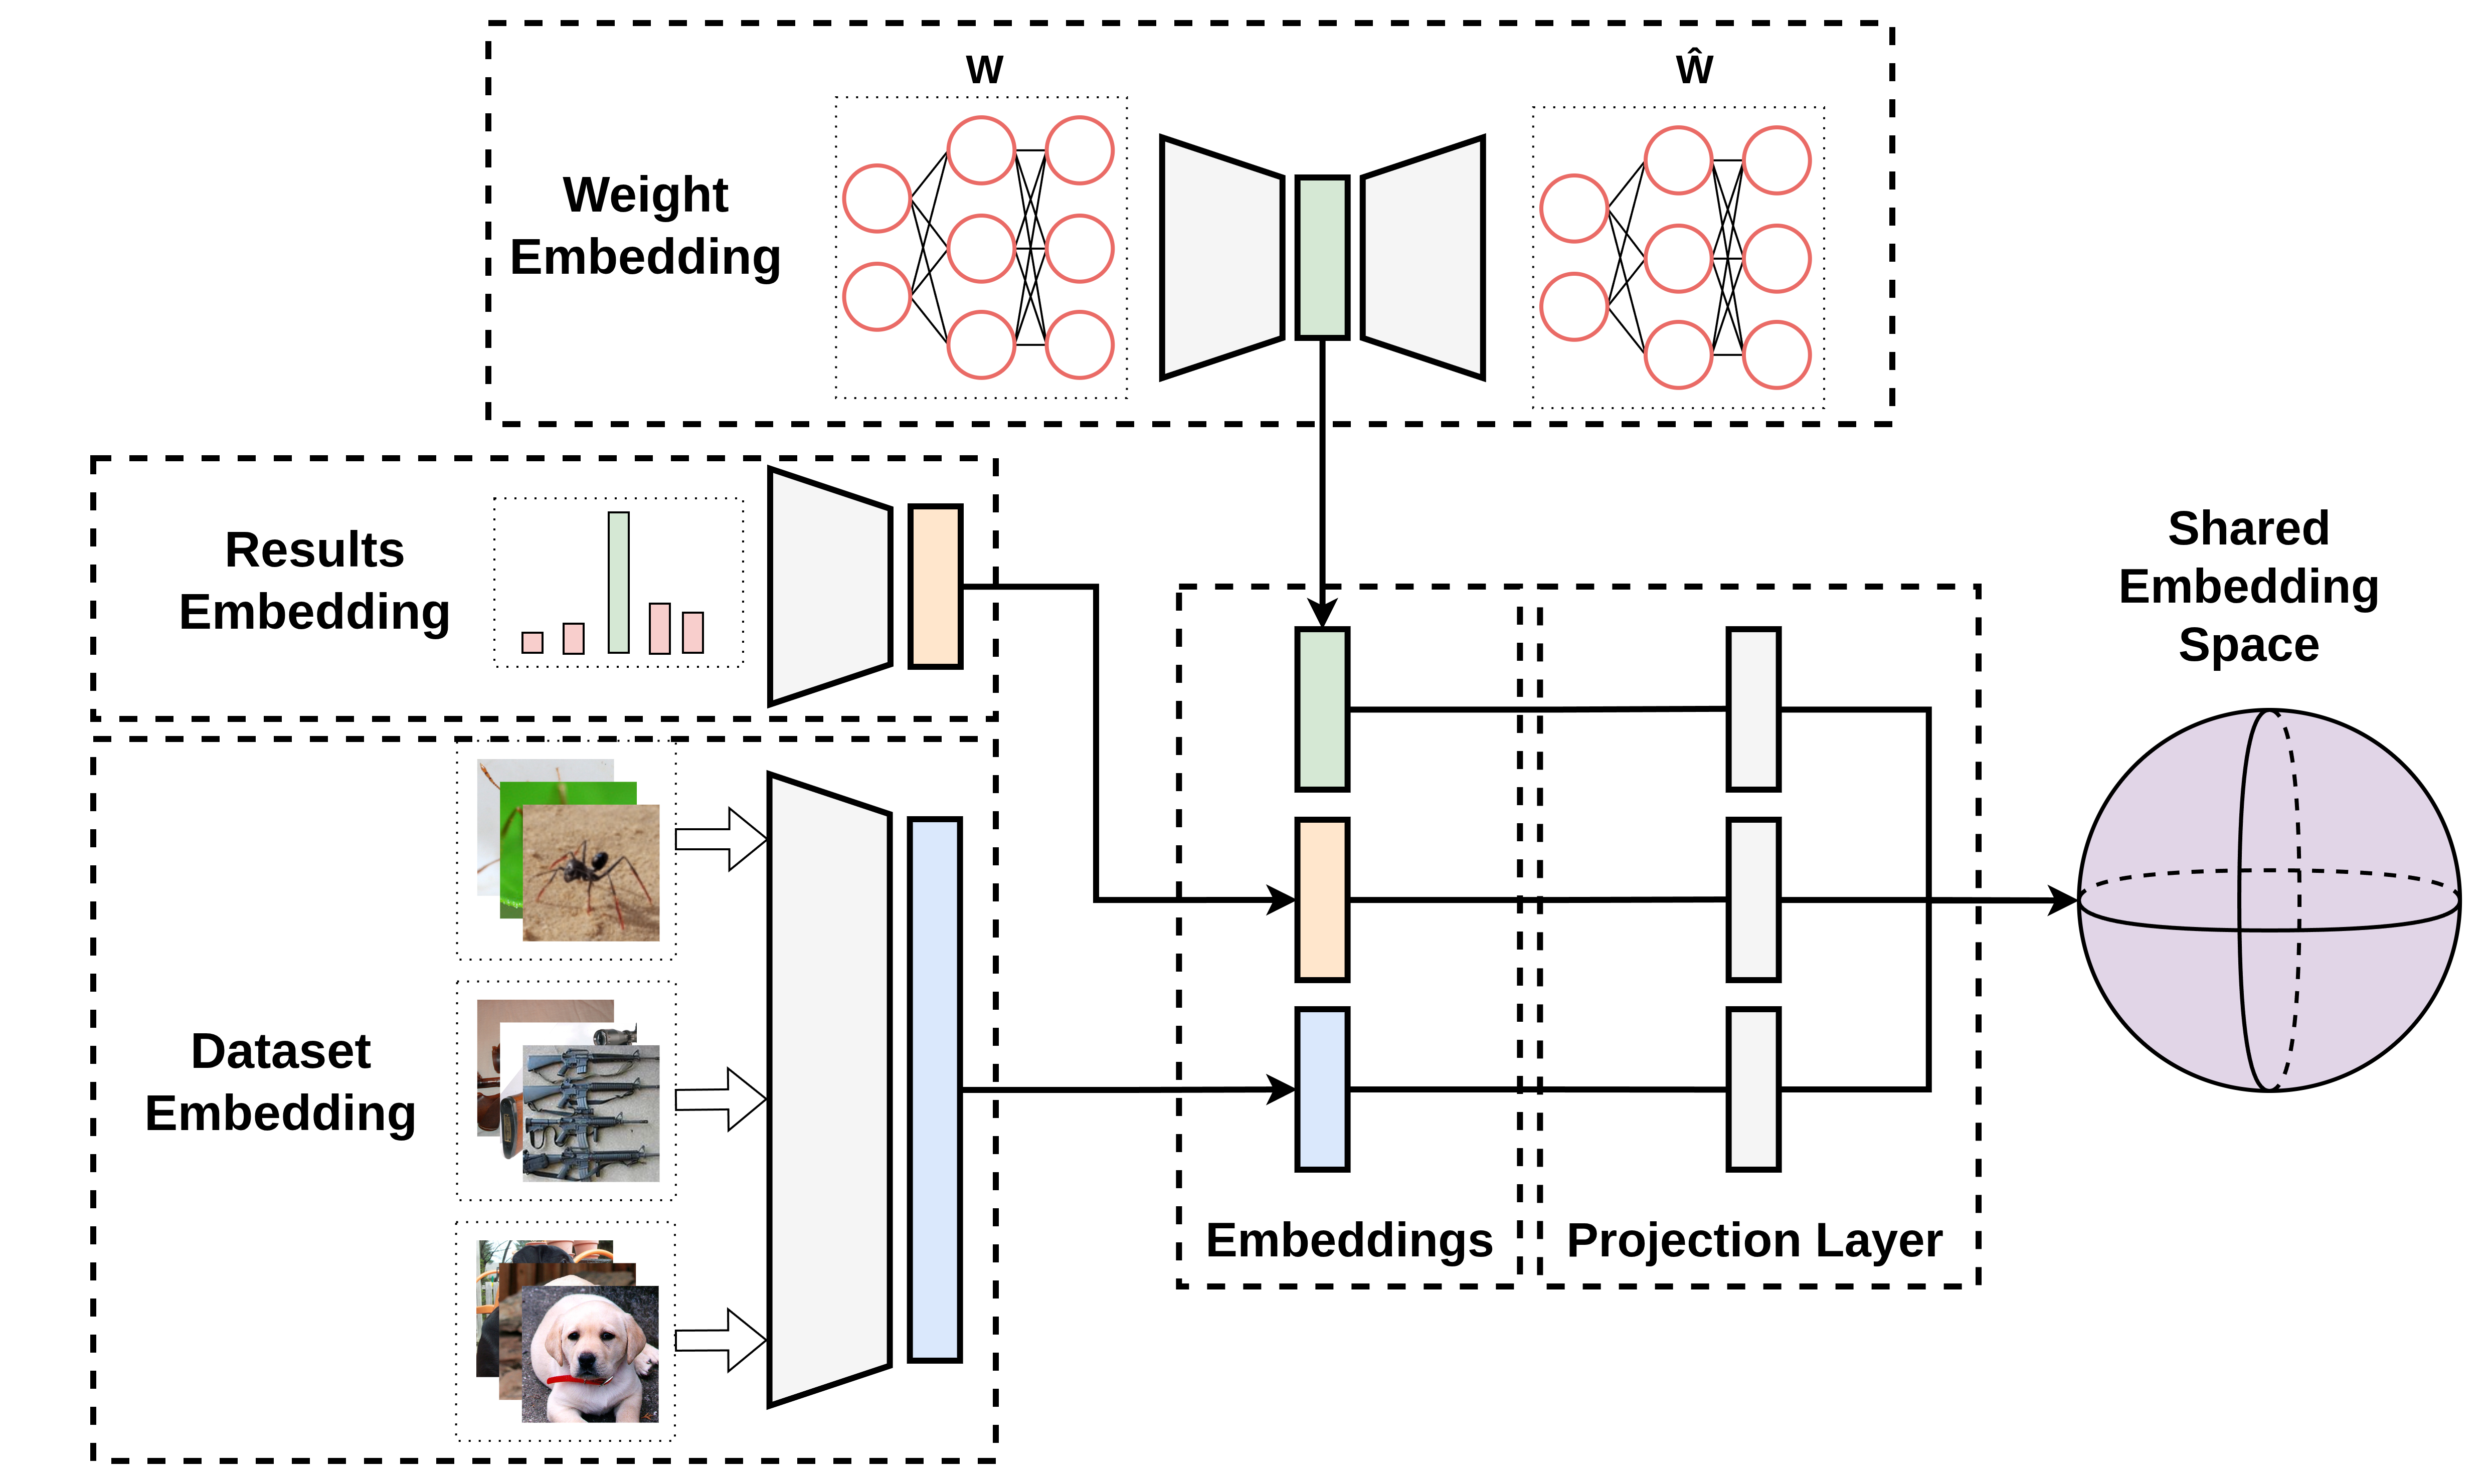
\includegraphics[width=0.75\linewidth]{pipeline.png}
    \caption[A figure illustrating the process of embedding a dataset, model weigths and results into a shared embedding space ]{AA figure illustrating the process of embedding a dataset, model weights and results in a shared embedding space. }
    \label{fig:pipeline}
\end{figure}

In this we report we develop a contrastive learning framework to create a unified embedding space that jointly represents neural network weights $(W)$, the datasets they were trained on $(\mathcal{D})$, and their resulting performance characteristics $(R)$.  Specifically, we construct two separate encoders—one for dataset embeddings using pre-trained CLIP features and one for weight embeddings using an autoencoder [cite] architecture, while creating a binned result embedding table, and train these encoders using a contrastive objective, NXTEnt \cite{agren2022ntxentlossupperbound}, that encourages related triplets $(\mathcal{D}, W, R)$ to be proximal in the shared latent space. Figure \ref{fig:pipeline} depicts a high-level view of the full embedding pipeline.

% TODO {introduction}

Our central hypothesis is that this unified representation space will enable two key capabilities:

Interpretability and Analysis: By examining the geometric relationships in the shared embedding space, we can better understand how dataset characteristics influence the learned weights and resulting model behaviors. This includes investigating questions such as: Do models trained on similar datasets cluster together in weight space? Can we identify which data characteristics most strongly determine weight patterns? 

Conditional Model Sampling: The learned distribution can enable sampling of model weights conditioned on both desired dataset properties and target performance metrics—that is, approximating P(W|D,R)—which could allow for more efficient model generation than training from scratch.







The results found from the report, and how it's limited 

The remainder of this report is structured as follows.:
    % TODO {outline_paragraph}
    In Section 1 we will discuss x, next y, concluded by z in attempt to showcase that this report is the best
    % TODO {outline_paragraph}
% TODO {introduction}


% \section{Section heading}

% This is some section with two table in it: Table~\ref{tbl:exemplars} and Table~\ref{tbl:abx_speaker}.

% \begin{table}[!h]
%     \mytable
%     \caption{Performance of the unconstrained segmental Bayesian model on TIDigits1 over iterations in which the reference set is refined.}
%     \begin{tabularx}{\linewidth}{@{}lCCCCC@{}}
%         \toprule
%         Metric     & 1 & 2 & 3 & 4 & 5 \\
%         \midrule
%         WER (\%)                        & $35.4$ & $23.5$ & $21.5$ & $21.2$ & $22.9$ \\
%         Average cluster purity (\%)       & $86.5$ & $89.7$ & $89.2$ & $88.5$ & $86.6$ \\
%         Word boundary $F$-score (\%)         & $70.6$ & $72.2$ & $71.8$ & $70.9$ & $69.4$ \\
%         Clusters covering 90\% of data   & 20             & 13 & 13 & 13 & 13 \\
%         \bottomrule
%     \end{tabularx}
%     \label{tbl:exemplars}
% \end{table}


% \begin{table}[!h]
%     \renewcommand{\arraystretch}{1.1}
%     \centering
%     \caption{A table with an example of using multiple columns.}
%     \begin{tabularx}{0.65\linewidth}{@{}lCCr@{}}
%         \toprule
%         & \multicolumn{2}{c}{Accuracy (\%)} \\
%         \cmidrule(lr){2-3}
%         Model    & Intermediate & Output & Bitrate\\
%         \midrule
%         Baseline & 27.5         & 26.4   & 116 \\
%         VQ-VAE   & 26.0         & 22.1   & 190 \\
%         CatVAE   & 28.7         & 24.3   & 215 \\
%         \bottomrule
%     \end{tabularx}
%     \label{tbl:abx_speaker}
% \end{table}

% \newpage

% This is a new page, showing what the page headings looks like, and showing how to refer to a figure like Figure~\ref{fig:cae_siamese}.

% \begin{figure}[!t]
%     \centering
% %     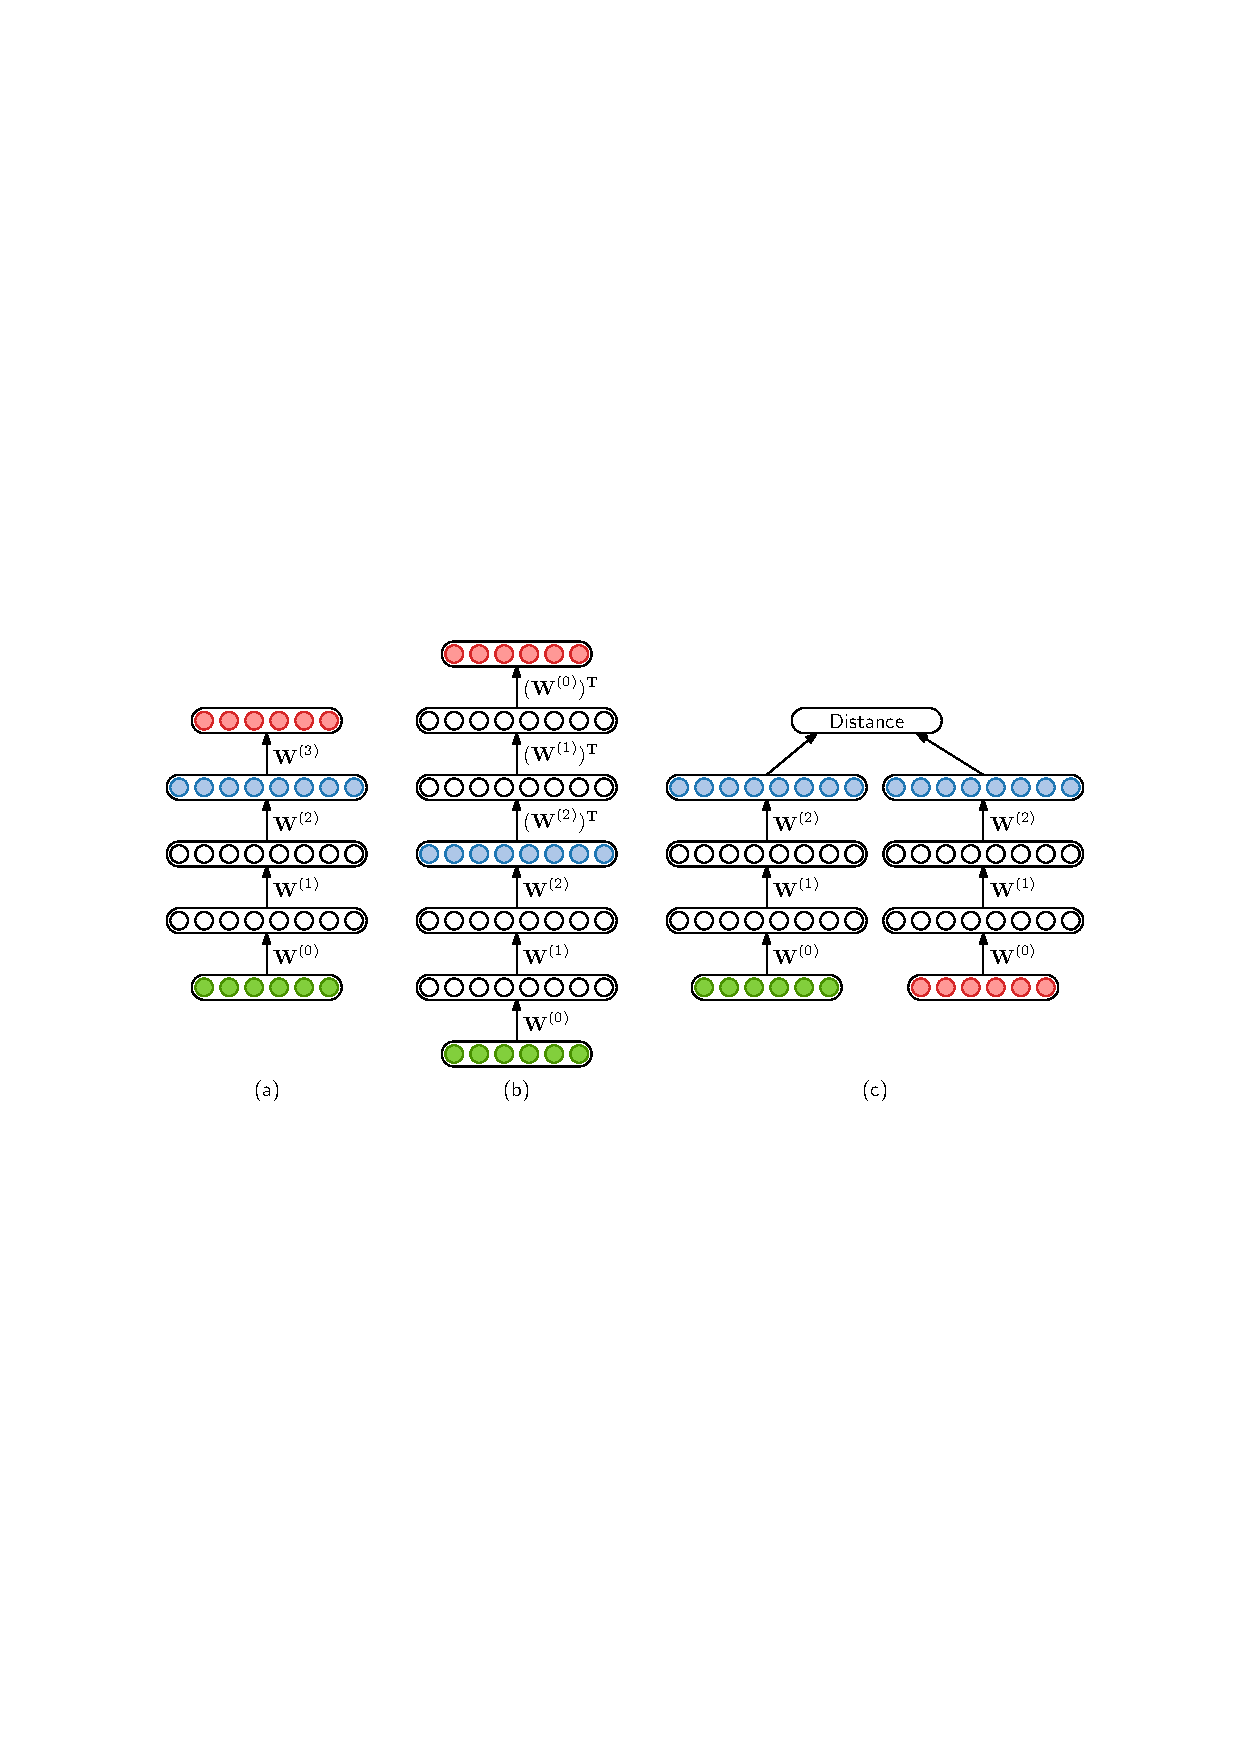
\includegraphics[width=\linewidth]{cae_siamese}
%     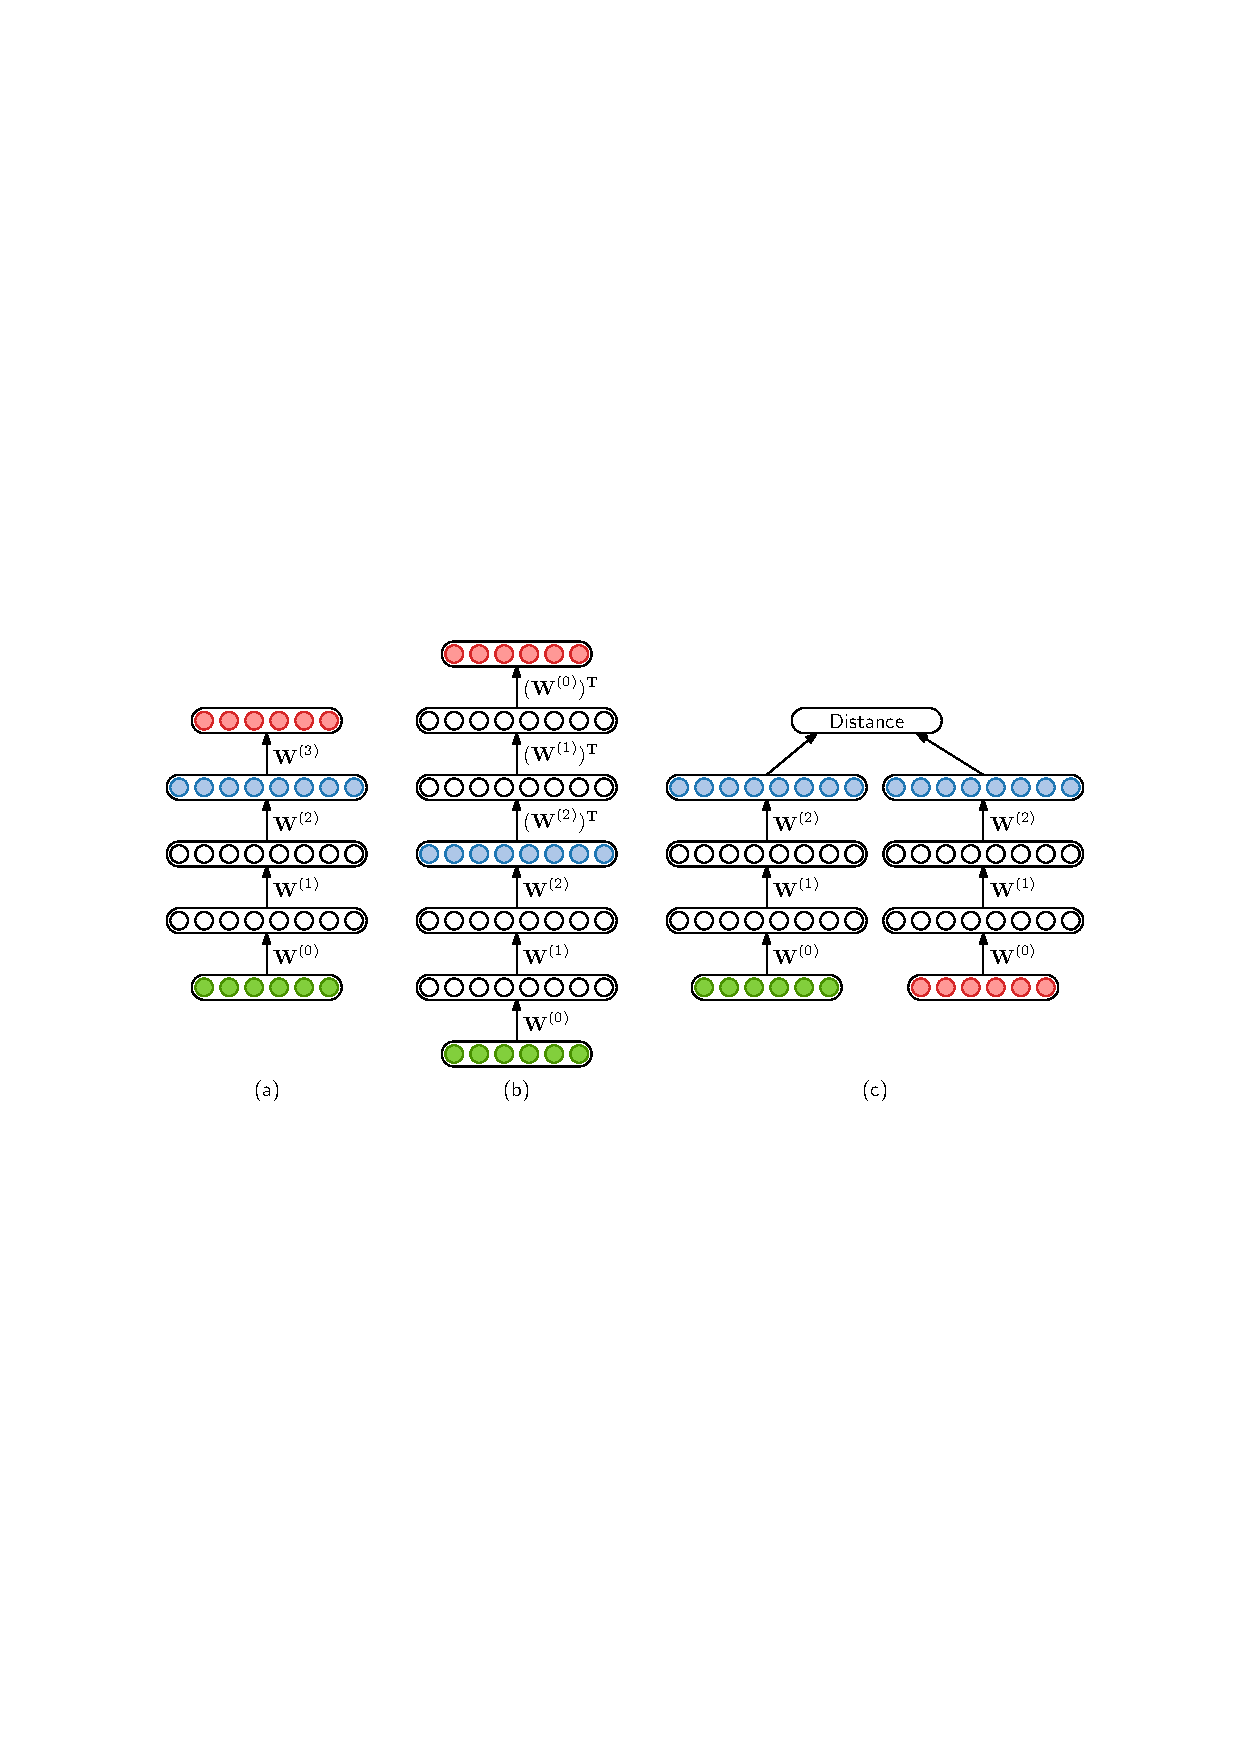
\includegraphics[width=0.918\linewidth]{cae_siamese}
%     \caption[I am the short caption that appears in the list of figures, without references.]{
%     (a) The cAE as used in this chapter. The encoding layer (blue) is chosen based on performance on a development set.
%     (b) The cAE with symmetrical tied weights. The encoding from the middle layer (blue) is always used.
%     (c) The siamese DNN. The cosine distance between aligned frames (green and red) is either minimized or maximized depending on whether the frames belong to the same (discovered) word or not.
%     A cAE can be seen as a type of DNN~\cite{dahl+etal_taslp12}.
%     }
%     \label{fig:cae_siamese}
% \end{figure}


% The following is an example of an equation:
% \begin{equation}
% P(\vec{z} | \vec{\alpha}) = \int_{\vec{\pi}} P(\vec{z} | \vec{\pi}) \, p(\vec{\pi} | \vec{\alpha}) \, \textrm{d} \vec{\pi}
% = \int_{\vec{\pi}} \prod_{k = 1}^K \pi_k^{N_k} \frac{1}{B(\vec{\alpha})} \prod_{k = 1}^K \pi_k^{\alpha_k - 1} \, \textrm{d} \vec{\pi}
% \label{eq:example_equation}
% \end{equation}
% which you can subsequently refer to as~\eqref{eq:example_equation} or Equation~\ref{eq:example_equation}.
% But make sure to consistently use the one or the other (and not mix the two ways of referring to equations).


